\chapter{Geodatabase Creation}
\section{Objective of the exercise}
Spatial files can be managed as individual files such as shapefiles or as a database. ArcGIS supports Geodatabase for management of data in a form of database.

\section{Data}
Use the \emph{tamakoshi.tif} map which is in the \emph{georefer} folder after georeferencing it.

\section{Steps}
\subsection{Creating Geodatabase}
\begin{enumerate}
\item{Open ArcMap}
\item{Open Catalog from main menu Windows | Catalog}
\item{Open a folder connection to the folder where you wish to save the geodatabase as presented in the Figure \ref{fig:geodatabase_folder_connection}}
	\begin{figure}[h]
	\centering
	\label{fig:geodatabase_folder_connection}
	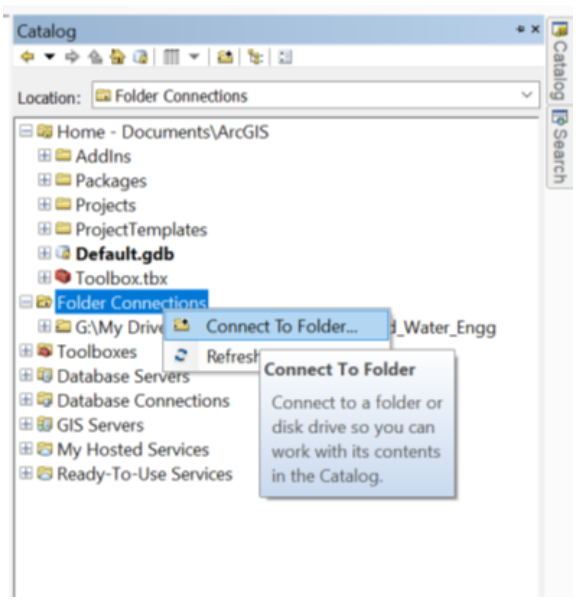
\includegraphics[scale=0.5]{images/geodatabase_folder_connection}
	\caption{Folder Connection to create Geodatabase}
	\label{fig:geodatabase_folder_connection}
	\end{figure}
\item{Once a Folder Connection is done, Right click on the Folder | New | File Geodatabase. Provide a suitable name to the geodatabase.}
\item Right click on the File Geodatabase | New | Feature Dataset
\item Select or import NEPAL\textunderscore MUTM\textunderscore CM\textunderscore 87\textunderscore EVEREST\textunderscore 1830 as coordinate system
\item Continue and Finish
\item Now go to the just created Feature Dataset | New | Feature
Class. Give a name and select the type of feature class. For now
select Point as type. Continue and finish.
\item Create two more Feature Class with types Line and Polygon.
\end{enumerate}

\subsection{Editing Features}
\begin{enumerate}
	\item Add the \emph{Georeferenced Tamakosh	i.tif} map
	\item Open the editor toolbar from \emph{Customize | Toolbar | Editor}
	\item Select the feature class you want to edit
	\item Now start to \emph{digitize} over the georeferenced map.
	\item After completion, press \emph{F2} to save the edits or you can select \emph{Editor | Save Edits}
		\item When you are done, select \emph{Editor - Stop edits}. When promted select \emph{Save the edits}.
	\item Now edit other feature classes. You must edit at least a point layer, one line layer and a polygon layer.
\end{enumerate}

\subsection{Exercise}
You are assigned to digitize River, House and Landuse layer from the lamabagar.tif map. Create a geodatabase then a feature dataset. Assign coordinate system as in earlier exercise. Now digitize the layers.

